\subsection{Messung der PSF}
Zur Bestimmung der Form der PSF werden Aufnahmen, der xy-, xz, und yz-Ebene der Golbeads verwendet. 
Dabei wird jeweils die Ausdehnung des Bildes in x-,y- und z-Richtung bestimmt.
Da die Goldkügelchen in erster Näherung als rund angenommen werden können, ist die Form der PSF theoretisch bekannt.
Sie folgt der Besselfunktion $J_1$, für die Beugung von Licht an einer Kreisblende.
Dieses Interferenzmuster kann angenähert werden durch die Funktion \ref{eq:psfapprox}
\begin{align}
	f(x)=I_0 \cdot \exp \left( -k \cdot x^2 \right) \cdot \cos \left(-\omega\cdot x\right). \label{eq:psfapprox}
\end{align}
\\ 
Die Ausdehnung der Airyscheibe entspricht nach dem Rayleigh-Kriterium dem Abstand der beiden ersten Minima voneinander. 
Durch (\ref{eq:psfapprox}) ist der Abstand des ersten Minimums vom ersten Maximum eindeutig mit dem Parameter $w$ bestimmt als:
\begin{align}
x_{min} = \frac{\pi}{2}\omega.
\end{align}
Die PSF wird mit ImageJ vermessen indem das Profil entlang der jeweiligen Achse durch das Maximum bestimmt wird.
In Abb. \ref{fig:psffits} sind die alle Vermessungen der PSF zu sehen. In Tab. \ref{tab:psffits} sind die durch nonlinear-regression bestimmten Werte aufgetragen, der Fehler ergibt sich aus der bei der Regression auftretenden Standartabweichung.
\\
Die aus dem Aufbau nach Gleichung (\ref{eq:airy-disc}) bestimmte Airyscheibe hat einen Durchmesser von 557.7~nm für eine Wellenlänge von 640~nm und 675.4~nm für eine Wellenlänge von 775~nm.
\\
Bei der Messung der Auslöschung der FLuoreszenz durch den STED-Laser wird eine konfokale Lochblende mit einem Durchmesser von 62.5~$\mu$m und einer 100-fachen Vergrößerung des Bildes benutzt. 
Dies entspricht dem 1.12-fachen Durchmesser der Airyscheibe für 640~nm und 0.92-fachen Durchmesser der Airyscheibe für 775~nm.
\begin{figure}
	\centering
	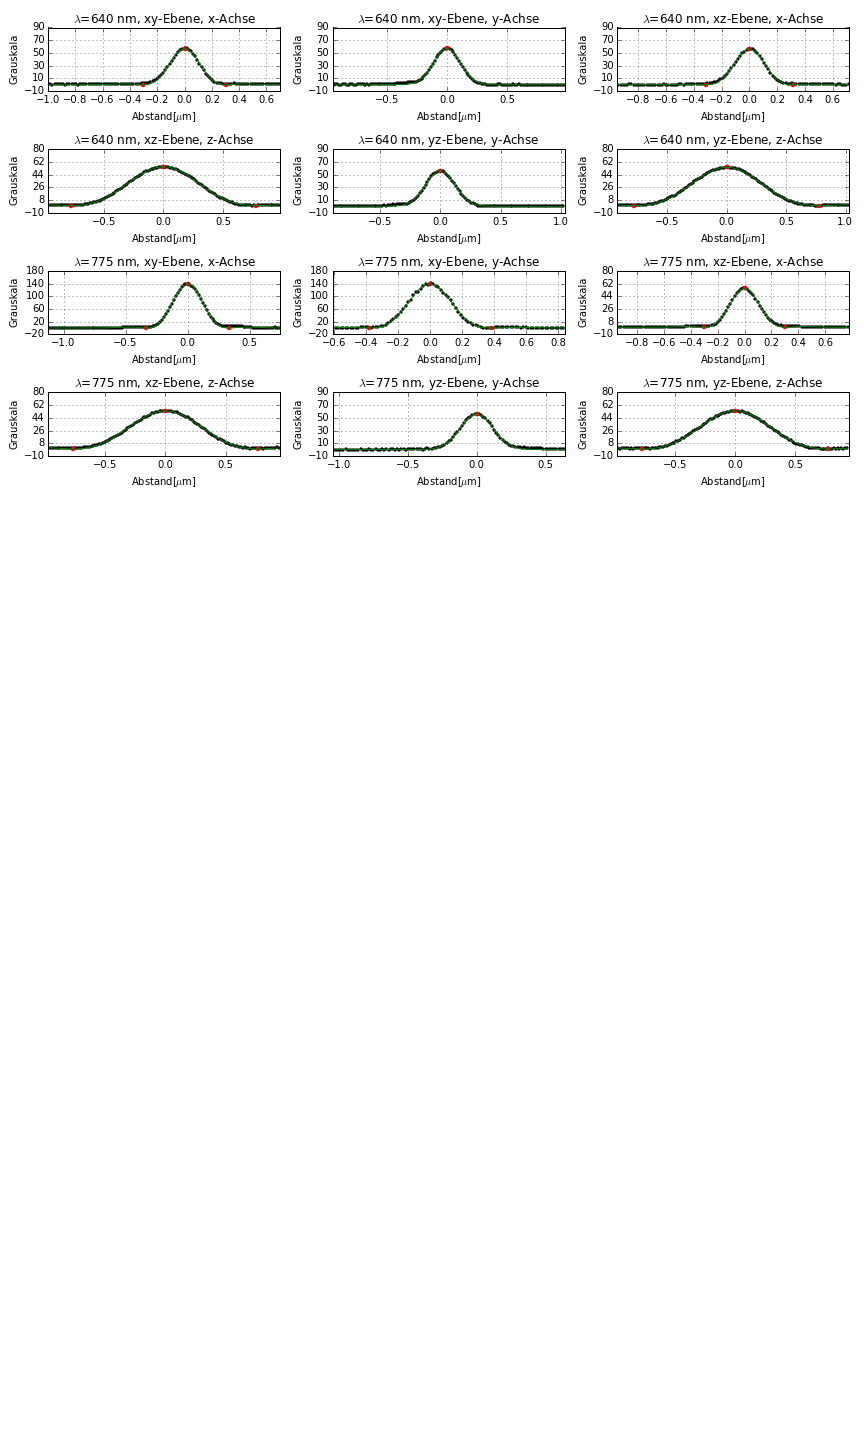
\includegraphics[trim= 0 950 0 0, width=\textwidth]{plots/goldbeads.png}
	\caption{Verteilung der Intensität der Aufnahmen, als Funktion des Abstandes vom ersten Maximum. Mit ImageJ bestimmte Werte sind schwarz dargestellt. 
		Maxima und erste Minima sind in rot hervorgehoben. 
		Die gefittete Funktion (grün) entspricht Gleichung (\ref{eq:psfapprox}). 
		Für die Messungen der y-Achse für die Wellenlängen 640~nm und 775~nm, liefert diese Methode der bestimmung der Minima keine sinnvollen Ergebnisse.
	}\label{fig:psffits}
\end{figure}

\begin{table}
	\centering
	\caption{Ergebnisse der nonlinear-regression für den Abstand der ersten Minima von einander, für jede Messung.
	Die Fehler ergeben sich aus der Standardabweichung der Messwerte von der mit der Regression bestimmten Kurve.
Für die $y$-Achsen Messwerte ist der Fehler der Regression viel größer als der bestimmte Durchmesser, der weit außerhalb der betrachteten Region liegen würde. }
	% Python latex table
	\begin{tabular}{l|l|l|c}
		Wellenlänge~[nm] & Ebene & Achse & Durchmesser der Airyscheibe~[$\mu$m] \\ \hline 
		640 & xy & x  &  0.604(6.0)\\ 
		 &  & y  &  0.0(100000000.0)\\ 
		 & xz & x  &  0.626(9.0)\\ 
		 &  & z  &  1.559(6.0)\\ 
		 & yz & y  &  0.0(100000000.0)\\ 
		 &  & z  &  1.555(6.0)\\ 
		775 & xy & x  &  0.668(6.0)\\ 
		 &  & y  &  0.761(8.0)\\ 
		 & xz & x  &  0.611(6.0)\\ 
		 &  & z  &  1.53(9.0)\\ 
		 & yz & y  &  0.0(100000000.0)\\ 
		 &  & z  &  1.546(8.0)\\ \hline
		640 &Gesamt & x & 0.610(5)\\
		    &	&y& --\\ 
		    &	&z& 1.557(4)\\
		775 &	&x& 0.639(5)\\
		    &	&y& 0.761(8)\\
		    &	&z& 1.546(8)\\
	\end{tabular}\label{tab:psffits}

\end{table}

\subsection{Tiefendiskriminierung}
In Abb. \ref{fig:tiefe} ist der Intensitätsverlauf in Abhängigkeit von der $z$-Achse entlang der Farbfilmprobe dargestellt.

\begin{figure}
	\centering
	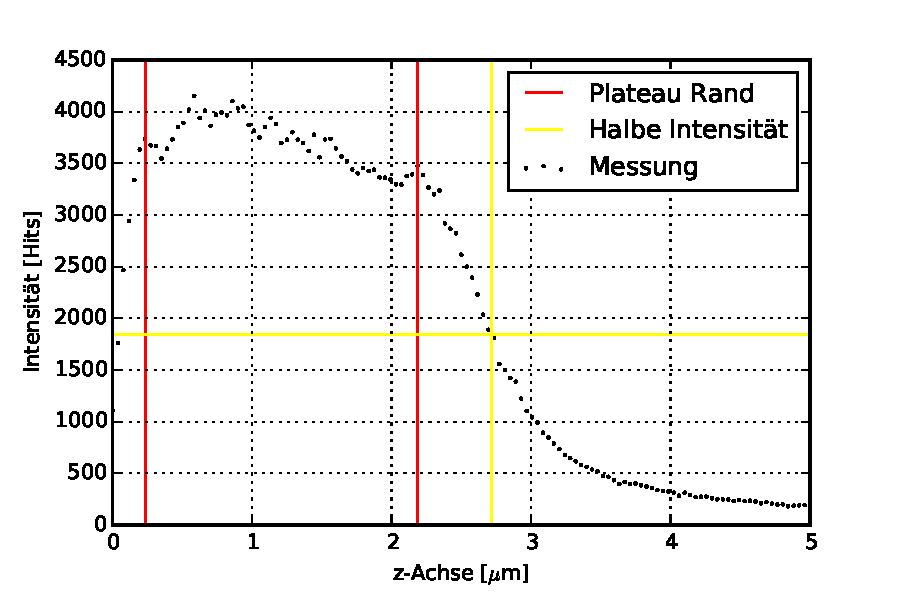
\includegraphics[width=\textwidth]{plots/tiefe.pdf}
	\caption{Verlauf der gemessenen Intensität beim Scannen des Farbfilms entlang der $z$-Achse. Die Intensität entspricht der Anzahl der detektierten Photonen im Photomultiplier.
	}\label{fig:tiefe}
\end{figure}

\subsection{STED-Auslöschung}
Zur Bestimmung der Sättigungsintensität $I_S$ wurde die Auslöschung, der durch den Anregungslaser erzeugten Fluoreszenz durch den STED-Laser bestimmt. 
Das Verhältnis zwischen Intensität des Anregungslasers und Restintensität ist in Abb. \ref{fig:depletion} dargestellt.
Die Fehler der Messung werden als die Standardabweichung der Messwerte für eine gegebene STED-Leistung und Beleuchtung angenommen.

Die Sättigungsintesität wird durch einen Fit der Funktion
\begin{align}
	f(x) = A \cdot \exp \left( -k \cdot x  \right).
\end{align}
bestimmt.
Für die Sättigungsintensität gilt:
\begin{align}
	I_{S} = \frac{\log 2}{k}.
\end{align}
Der über die Regression bestimmte Wert liegt bei 3.08(1)~mW.

\begin{figure}
	\centering
	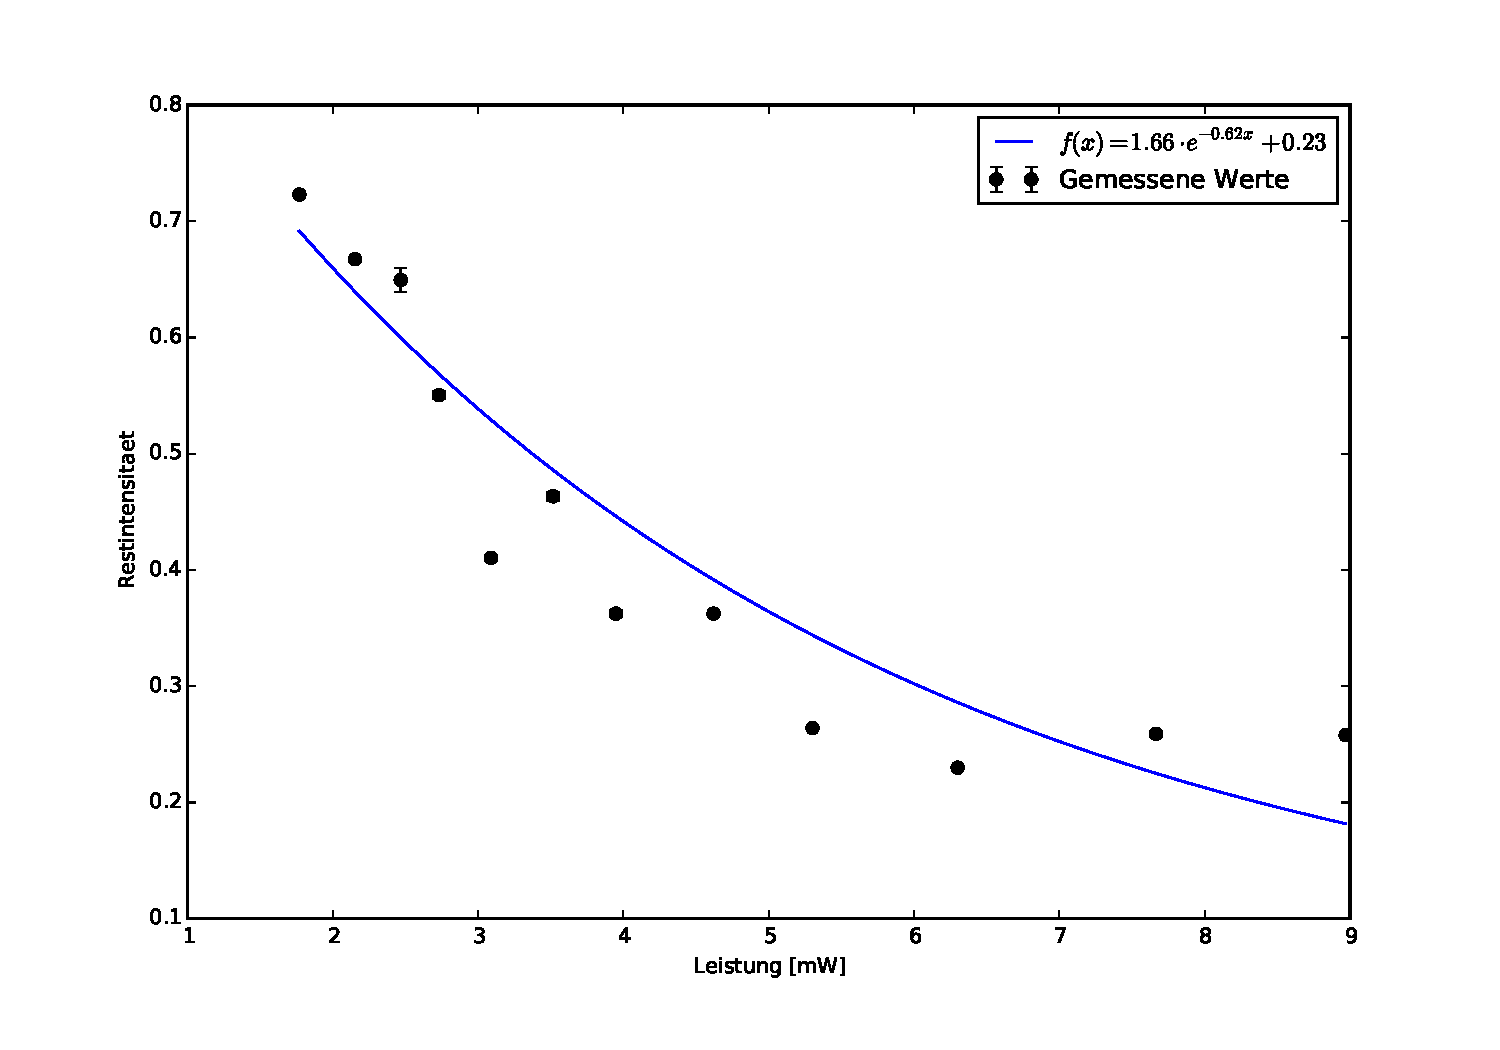
\includegraphics[width=\textwidth]{plots/depletion.pdf}
	\caption{Restintensität als Anteil der Anregungsintensität für verschiedene STED-Leistungen. 
		Die Fehlerbalken ergeben sich aus der Standardabweichung der einzelnen Messungen für eine gegebene STED-Leistung und Beleuchtungsart. 
		Die Messung der Intensität bei Beleuchtung duch den Anregungslaser allein ergibt vier Messwerte je STED-Leistung, und die Messung der Intensität bei gleichzeitiger Beleuchtung mit Anregungs- und STED-Laser liefert zwei Messwerte.
	Die Kurve folgt einem exponentiellen Abfall mit Abfallrate $k=0.23$~[mW]$^{-1}$. 
Die dadurch bestimmte Sättigungsintensität ist 3.08(1)~mW.}\label{fig:depletion}
\end{figure}


